\begin{figure}
    \centering
    \setlength{\tabcolsep}{1pt}
    {\small
    \begin{tabular}{ccccc}
        & Input & W/o text  & W/o diverse & Full method \\
        && prompt & lighting \\
        %
        \raisebox{35pt}{\rotatebox[origin=c]{90}{View 1}} &
        \multicolumn{1}{c}{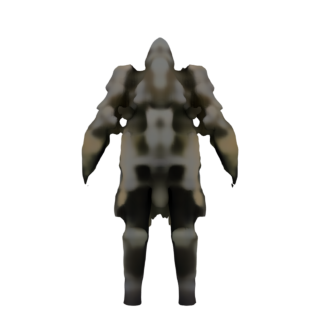
\includegraphics[width=0.24\linewidth, trim=50 0 50 0, clip]{images/ablation_plot/shap_e/mv_0_image_tile_1.png}} &
        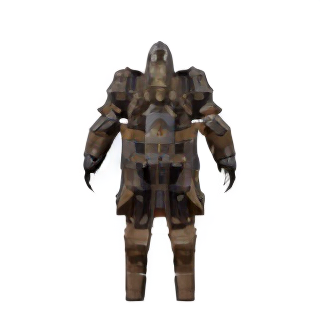
\includegraphics[width=0.24\linewidth, trim=50 0 50 0, clip]{images/ablation_plot/no_prompt/no_prompt_tile_1.png} &
        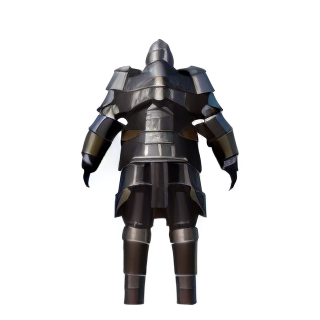
\includegraphics[width=0.24\linewidth, trim=50 0 50 0, clip]{images/ablation_plot/single_hdr/single_source_tile_1.png} &
        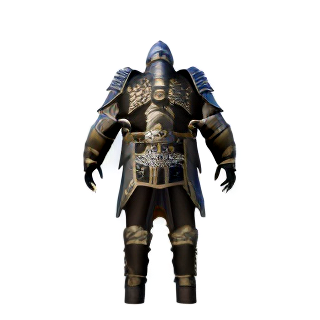
\includegraphics[width=0.24\linewidth, trim=50 0 50 0, clip]{images/ablation_plot/full/full_tile_1.png} \\
        %
        \raisebox{35pt}{\rotatebox[origin=c]{90}{View 2}} &
        \multicolumn{1}{c}{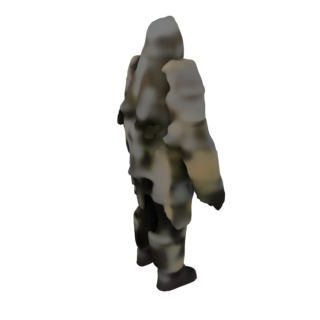
\includegraphics[width=0.24\linewidth, trim=50 0 50 0, clip]{images/ablation_plot/shap_e/mv_0_image_tile_2.png}} &
        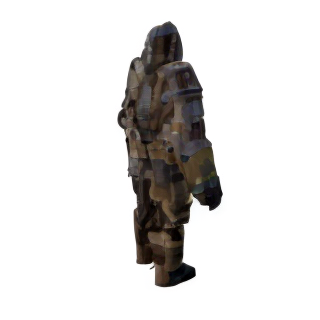
\includegraphics[width=0.24\linewidth, trim=50 0 50 0, clip]{images/ablation_plot/no_prompt/no_prompt_tile_2.png} &
        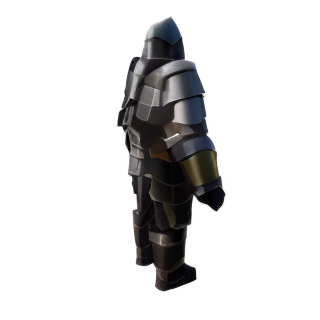
\includegraphics[width=0.24\linewidth, trim=50 0 50 0, clip]{images/ablation_plot/single_hdr/single_source_tile_2.png} &
        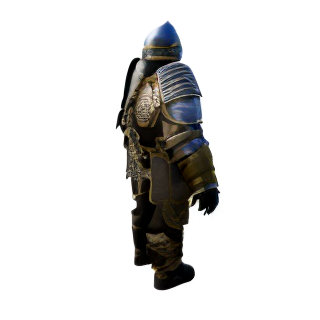
\includegraphics[width=0.24\linewidth, trim=50 0 50 0, clip]{images/ablation_plot/full/full_tile_2.png} \\
        %
        \raisebox{35pt}{\rotatebox[origin=c]{90}{View 3}} &
        \multicolumn{1}{c}{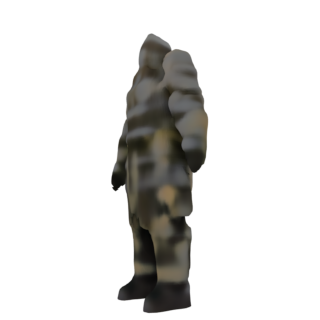
\includegraphics[width=0.24\linewidth, trim=50 0 50 0, clip]{images/ablation_plot/shap_e/mv_0_image_tile_5.png}} &
        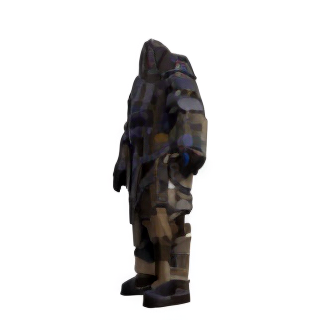
\includegraphics[width=0.24\linewidth, trim=50 0 50 0, clip]{images/ablation_plot/no_prompt/no_prompt_tile_5.png} &
        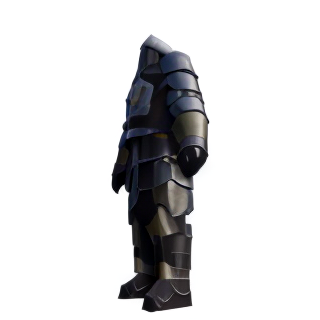
\includegraphics[width=0.24\linewidth, trim=50 0 50 0, clip]{images/ablation_plot/single_hdr/single_source_tile_5.png} &
        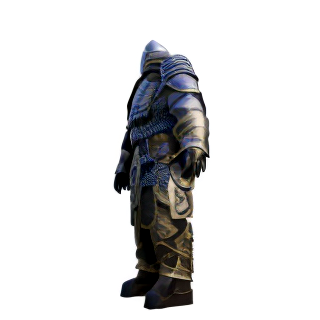
\includegraphics[width=0.24\linewidth, trim=50 0 50 0, clip]{images/ablation_plot/full/full_tile_5.png} \\
        %
        \multicolumn{5}{c}{``A knight in full plate armor''}
    \end{tabular}
    }
    \caption{Qualitative ablation study. The first column shows the degraded input object generated by Shap-E. Subsequent columns show the effects of removing specific components: omitting the text prompt leads to reduced texture detail, while excluding diverse lighting results in a flatter appearance with less realistic shading. The full model achieves the most refined and detailed result.}
    \label{fig:ablation}
\end{figure}
